% Digital Timing Diagram
% Demonstrates: clock, data, enable, and output waveforms with TikZ.
% Compile with: pdflatex main.tex

\documentclass[border=10pt]{standalone}
\usepackage{tikz}
\usetikzlibrary{arrows.meta, calc}

\begin{document}
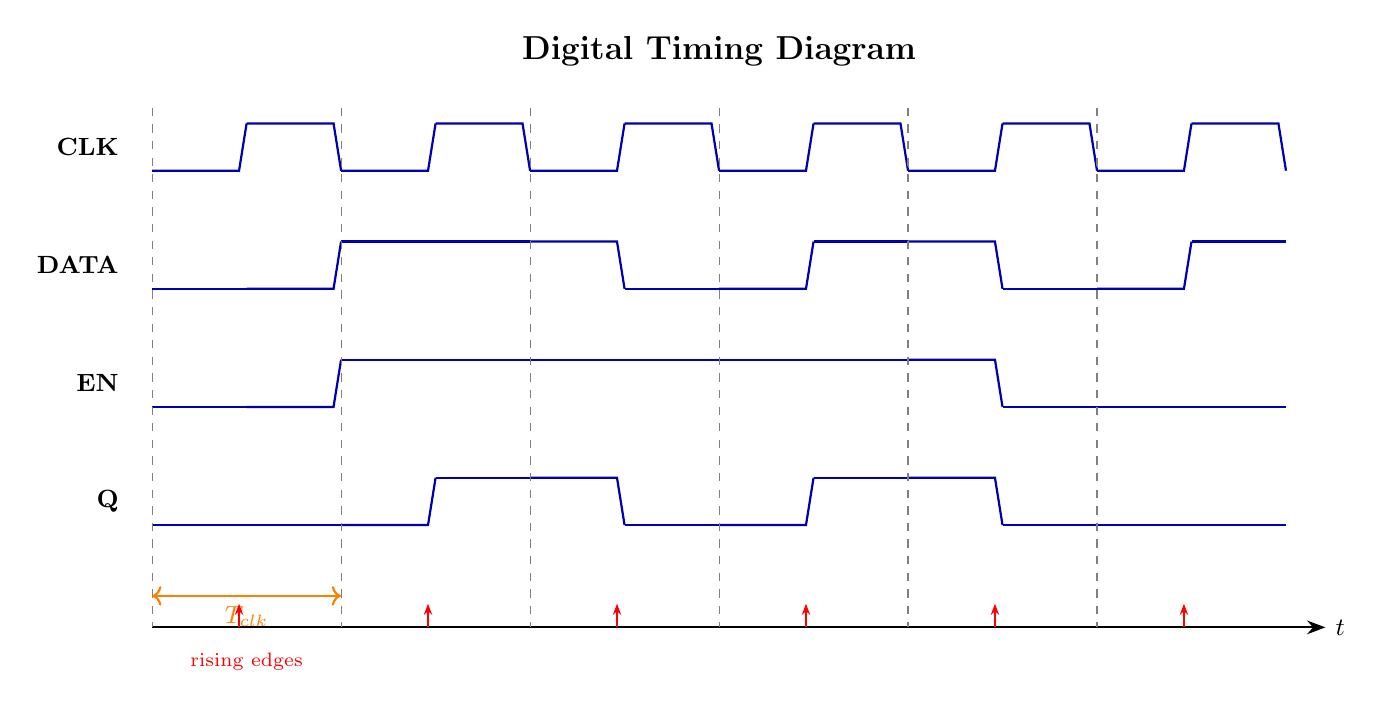
\begin{tikzpicture}[
    signal/.style={thick},
    hline/.style={thick, blue!70!black},
    lline/.style={thick, blue!70!black},
    trans/.style={thick, blue!70!black},
    label/.style={font=\bfseries\small, anchor=east},
]

% Configuration
\def\bitw{1.2}     % width of one clock period
\def\high{0.6}     % height of logic high
\def\sep{1.5}      % vertical separation between signals
\def\rise{0.08}    % rise/fall time (fraction of bitw)

% Helper: draw one bit (low=0, high=1)
% #1=x start, #2=y base, #3=value (0 or 1), #4=next value (for transition)
\newcommand{\drawbit}[4]{
    \pgfmathsetmacro{\yval}{#2 + #3*\high}
    \pgfmathsetmacro{\ynext}{#2 + #4*\high}
    \draw[trans] (#1, \yval) -- ({#1+\bitw*(1-\rise)}, \yval)
                 -- ({#1+\bitw}, \ynext);
}

% =============================================================================
% Signal: CLK (clock)
% =============================================================================
\def\yClk{0}
\node[label] at (-0.3, {\yClk+\high/2}) {CLK};

\foreach \i/\v/\n in {
    0/0/1, 1/1/0, 2/0/1, 3/1/0, 4/0/1, 5/1/0,
    6/0/1, 7/1/0, 8/0/1, 9/1/0, 10/0/1, 11/1/0
} {
    \drawbit{\i*\bitw}{\yClk}{\v}{\n}
}

% =============================================================================
% Signal: DATA
% =============================================================================
\def\yData{-1.5}
\node[label] at (-0.3, {\yData+\high/2}) {DATA};

\foreach \i/\v/\n in {
    0/0/0, 1/0/1, 2/1/1, 3/1/1, 4/1/0, 5/0/0,
    6/0/1, 7/1/1, 8/1/0, 9/0/0, 10/0/1, 11/1/1
} {
    \drawbit{\i*\bitw}{\yData}{\v}{\n}
}

% =============================================================================
% Signal: EN (enable)
% =============================================================================
\def\yEn{-3.0}
\node[label] at (-0.3, {\yEn+\high/2}) {EN};

\foreach \i/\v/\n in {
    0/0/0, 1/0/1, 2/1/1, 3/1/1, 4/1/1, 5/1/1,
    6/1/1, 7/1/1, 8/1/0, 9/0/0, 10/0/0, 11/0/0
} {
    \drawbit{\i*\bitw}{\yEn}{\v}{\n}
}

% =============================================================================
% Signal: Q (output = DATA AND EN, latched on rising CLK)
% =============================================================================
\def\yQ{-4.5}
\node[label] at (-0.3, {\yQ+\high/2}) {Q};

\foreach \i/\v/\n in {
    0/0/0, 1/0/0, 2/0/1, 3/1/1, 4/1/0, 5/0/0,
    6/0/1, 7/1/1, 8/1/0, 9/0/0, 10/0/0, 11/0/0
} {
    \drawbit{\i*\bitw}{\yQ}{\v}{\n}
}

% =============================================================================
% Time axis
% =============================================================================
\draw[-{Stealth}, thick] (0, -5.8) -- ({12*\bitw + 0.5}, -5.8)
    node[right, font=\small] {$t$};

% Clock period markers
\foreach \i in {0,2,...,10} {
    \draw[gray, thin, dashed] ({\i*\bitw}, 0.8) -- ({\i*\bitw}, -5.8);
}

% Period annotation
\draw[<->, thick, orange] ({0*\bitw}, -5.4) -- ({2*\bitw}, -5.4)
    node[midway, below, font=\small] {$T_{\text{clk}}$};

% Rising edge markers
\foreach \i in {0,2,...,10} {
    \draw[red, thick, -{Stealth[length=4pt]}]
        ({\i*\bitw + \bitw*0.92}, -5.8) -- ++(0, 0.3);
}
\node[red, font=\scriptsize, below] at ({1*\bitw}, -6) {rising edges};

% Title
\node[font=\bfseries\large, above] at ({6*\bitw}, 1.2) {Digital Timing Diagram};

\end{tikzpicture}
\end{document}
